\section{Background}

\subsection{LUKS2 Disk Encryption}
also \cite{Fruwirth2018}

\emph{Linux Unified Key Setup 2}, or short LUKS2, is the second version of a disk encryption standard. It provides a specification \cite{Broz2018} for a on-disk format for storing the encryption metadata as well as the encrypted user data. Unlocking an encrypted disk is achieved by providing one of possibly multiple passphrases or keyfiles. The intended usage of LUKS2 is together with the Linux dm-crypt subsystem, but that is not mandatory\footnote{\label{fn:luks2windows} As we show in this thesis it is possible to make the combination of LUKS2 and Windows work.}. The reference implementation\footnote{\label{f:luks2referenceimpl} \url{https://gitlab.com/cryptsetup/cryptsetup}} is designed only for usage on Linux, which is why we developed a new Rust library for interacting with LUKS2 partitions.

What are the differences between LUKS2 and LUKS? Besides new password hashing functions (I think)

Mention own \texttt{luks2} Rust crate

\subsubsection{On-Disk Format}
\begin{figure}[h]
	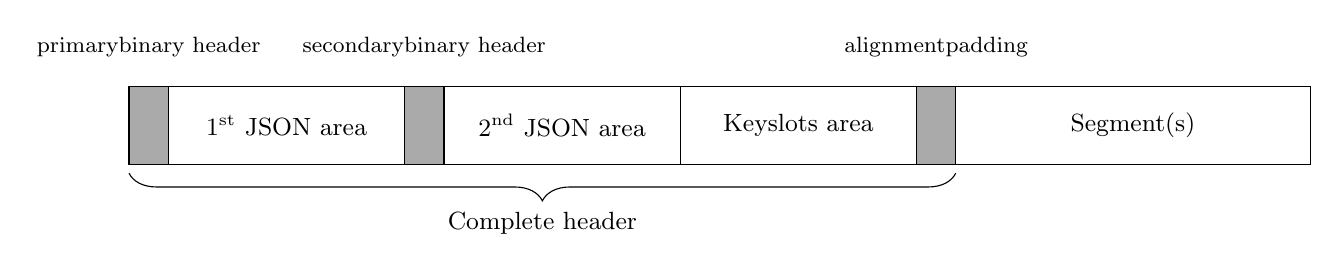
\begin{tikzpicture}
		\node [anchor=center] at (0.25, 1.5) {\footnotesize\makecell{primary\\binary header}};
		\draw [fill={rgb:black, 1; white, 2}] (0, 0) rectangle (0.5, 1);
		\draw [fill=white] (0.5, 0) rectangle (3.5, 1);
		\node [anchor=center] at (2, 0.5) {\small\makecell{1\textsuperscript{st} JSON area}};
		\node [anchor=center] at (3.75, 1.5) {\footnotesize\makecell{secondary\\binary header}};
		\draw [fill={rgb:black, 1; white, 2}] (3.5, 0) rectangle (4, 1);
		\draw [fill=white] (4, 0) rectangle (7, 1);
		\node [anchor=center] at (5.5, 0.5) {\small\makecell{2\textsuperscript{nd} JSON area}};
		\draw [fill=white] (7, 0) rectangle (10, 1);
		\node [anchor=center] at (8.5, 0.5) {\small\makecell{Keyslots area}};
		\node [anchor=center] at (10.25, 1.5) {\footnotesize\makecell{alignment\\padding}};
		\draw [fill={rgb:black, 1; white, 2}] (10, 0) rectangle (10.5, 1);

		\draw [decorate, decoration={brace, amplitude=10pt, mirror}, yshift=-3pt]
		(0, 0) -- (10.5, 0) node [black, midway, yshift=-18pt] {\small Complete header};

		\draw [fill=white] (10.5, 0) rectangle (15, 1);
		\node [anchor=center] at (12.75, 0.5) {\small\makecell{Segment(s)}};
	\end{tikzpicture}
	\caption[
		LUKS2 on-disk format
	]{
		LUKS2 on-disk format (modified after \cite{Broz2018}). The complete header consists of three areas: a binary header of exactly one 4096-byte sector, JSON metadata, and the binary keyslots data. A \emph{keyslot} is an ``encrypted area on disk that contains a key'' \cite{Broz2018}. For redundancy, the binary header and the JSON metadata are stored twice. After that follow one or areas containing encrypted user data. The specification calls these areas \emph{segments}.
	}
	\label{fig:luks2ondisk}
\end{figure}

Figure \ref{fig:luks2ondisk} shows the high-level layout of a LUKS2-encrypted disk.

The two binary headers have a size of exactly one sector, so that they are always written atomically. Only the first 512 bytes are actually used. The header marks the disk as following the LUKS2 specification and contains metadata such as labels, a UUID, and a header checksum. The labels and UUID can be accessed using the \texttt{blkid}\footnote{\label{fn:blkid} \url{https://linux.die.net/man/8/blkid}} command-line tool and also be used in the \texttt{udev}\footnote{\label{fn:udev} \url{https://linux.die.net/man/8/udev}} Linux subsystem. For the detailed contents see Figure \ref{fig:luks2binhdrstructure}. Figure \ref{fig:luks2binhdrexample} also contains an example hexdump of a binary header.

\begin{figure}[h]
	\begin{lstlisting}[style=CStyle]
#define MAGIC_1ST "LUKS\xba\xbe"
#define MAGIC_2ND "SKUL\xba\xbe"
#define MAGIC_L     6
#define UUID_L     40
#define LABEL_L    48
#define SALT_L     64
#define CSUM_ALG_L 32
#define CSUM_L     64

// All integers are stored as big-endian.
// Header structure must be exactly 4096 bytes.

struct luks2_hdr_disk {
    char magic[MAGIC_L];        // MAGIC_1ST or MAGIC_2ND
    uint16_t version;           // Version 2
    uint64_t hdr_size;          // size including JSON area [bytes]
    uint64_t seqid;             // sequence ID, increased on update
    char label[LABEL_L];        // ASCII label or empty
    char csum_alg[CSUM_ALG_L];  // checksum algorithm, "sha256"
    uint8_t salt[SALT_L];       // salt, unique for every header
    char uuid[UUID_L];          // UUID of device
    char subsystem[LABEL_L];    // owner subsystem label or empty
    uint64_t hdr_offset;        // offset from device start [bytes]
    char _padding[184];         // must be zeroed
    uint8_t csum[CSUM_L];       // header checksum
    char _padding4096[7*512];   // Padding, must be zeroed
} __attribute__((packed));
\end{lstlisting}
	\caption[
		LUKS2 binary header structure
	]{
		LUKS2 binary header structure from \cite{Broz2018}. Integers are stored in big-endian format, and all strings have to be null-terminated. The \texttt{magic}, \texttt{version}, and \texttt{uuid} fields are also present in the LUKS1 binary header and were placed at the same offsets as there.
	}
	\label{fig:luks2binhdrstructure}
\end{figure}

\begin{figure}
	\ttfamily
	\scriptsize
	\begin{tabular}{c|*{16}{c}|l}
		0000 & \cellcolor{tPink}4C & \cellcolor{tPink}55 & \cellcolor{tPink}4B & \cellcolor{tPink}53 & \cellcolor{tPink}BA & \cellcolor{tPink}BE & \cellcolor{tOrng}00 & \cellcolor{tOrng}02 & \cellcolor{tYlow}00 & \cellcolor{tYlow}00 & \cellcolor{tYlow}00 & \cellcolor{tYlow}00 & \cellcolor{tYlow}00 & \cellcolor{tYlow}00 & \cellcolor{tYlow}40 & \cellcolor{tYlow}00 & \coltxt{tPink}{LUKSº¾}\coltxt{tOrng}{..}\coltxt{tYlow}{......@.} \\
		0010 & \cellcolor{tGren}00 & \cellcolor{tGren}00 & \cellcolor{tGren}00 & \cellcolor{tGren}00 & \cellcolor{tGren}00 & \cellcolor{tGren}00 & \cellcolor{tGren}00 & \cellcolor{tGren}03 & \cellcolor{tLblu}54 & \cellcolor{tLblu}68 & \cellcolor{tLblu}69 & \cellcolor{tLblu}73 & \cellcolor{tLblu}20 & \cellcolor{tLblu}69 & \cellcolor{tLblu}73 & \cellcolor{tLblu}20 & \coltxt{tGren}{........}\coltxt{tLblu}{This is } \\
		0020 & \cellcolor{tLblu}61 & \cellcolor{tLblu}6E & \cellcolor{tLblu}20 & \cellcolor{tLblu}41 & \cellcolor{tLblu}53 & \cellcolor{tLblu}43 & \cellcolor{tLblu}49 & \cellcolor{tLblu}49 & \cellcolor{tLblu}20 & \cellcolor{tLblu}6C & \cellcolor{tLblu}61 & \cellcolor{tLblu}62 & \cellcolor{tLblu}65 & \cellcolor{tLblu}6C & \cellcolor{tLblu}00 & \cellcolor{tLblu}00 & \coltxt{tLblu}{an ASCII label..} \\
		0030 & \cellcolor{tLblu}00 & \cellcolor{tLblu}00 & \cellcolor{tLblu}00 & \cellcolor{tLblu}00 & \cellcolor{tLblu}00 & \cellcolor{tLblu}00 & \cellcolor{tLblu}00 & \cellcolor{tLblu}00 & \cellcolor{tLblu}00 & \cellcolor{tLblu}00 & \cellcolor{tLblu}00 & \cellcolor{tLblu}00 & \cellcolor{tLblu}00 & \cellcolor{tLblu}00 & \cellcolor{tLblu}00 & \cellcolor{tLblu}00 & \coltxt{tLblu}{................} \\
		0040 & \cellcolor{tLblu}00 & \cellcolor{tLblu}00 & \cellcolor{tLblu}00 & \cellcolor{tLblu}00 & \cellcolor{tLblu}00 & \cellcolor{tLblu}00 & \cellcolor{tLblu}00 & \cellcolor{tLblu}00 & \cellcolor{tBlue}73 & \cellcolor{tBlue}68 & \cellcolor{tBlue}61 & \cellcolor{tBlue}32 & \cellcolor{tBlue}35 & \cellcolor{tBlue}36 & \cellcolor{tBlue}00 & \cellcolor{tBlue}00 & \coltxt{tLblu}{........}\coltxt{tBlue}{sha256..} \\
		0050 & \cellcolor{tBlue}00 & \cellcolor{tBlue}00 & \cellcolor{tBlue}00 & \cellcolor{tBlue}00 & \cellcolor{tBlue}00 & \cellcolor{tBlue}00 & \cellcolor{tBlue}00 & \cellcolor{tBlue}00 & \cellcolor{tBlue}00 & \cellcolor{tBlue}00 & \cellcolor{tBlue}00 & \cellcolor{tBlue}00 & \cellcolor{tBlue}00 & \cellcolor{tBlue}00 & \cellcolor{tBlue}00 & \cellcolor{tBlue}00 & \coltxt{tBlue}{................} \\
		0060 & \cellcolor{tBlue}00 & \cellcolor{tBlue}00 & \cellcolor{tBlue}00 & \cellcolor{tBlue}00 & \cellcolor{tBlue}00 & \cellcolor{tBlue}00 & \cellcolor{tBlue}00 & \cellcolor{tBlue}00 & \cellcolor{tPurp}EB & \cellcolor{tPurp}0F & \cellcolor{tPurp}D2 & \cellcolor{tPurp}C6 & \cellcolor{tPurp}E3 & \cellcolor{tPurp}D2 & \cellcolor{tPurp}8D & \cellcolor{tPurp}4B & \coltxt{tBlue}{........}\coltxt{tPurp}{ë.ÒÆãÒ.K} \\
		0070 & \cellcolor{tPurp}BB & \cellcolor{tPurp}2B & \cellcolor{tPurp}8A & \cellcolor{tPurp}49 & \cellcolor{tPurp}E6 & \cellcolor{tPurp}2E & \cellcolor{tPurp}4E & \cellcolor{tPurp}B7 & \cellcolor{tPurp}04 & \cellcolor{tPurp}2F & \cellcolor{tPurp}A9 & \cellcolor{tPurp}39 & \cellcolor{tPurp}76 & \cellcolor{tPurp}71 & \cellcolor{tPurp}8F & \cellcolor{tPurp}8A & \coltxt{tPurp}{»+ŠIæ.N·./©9vq.Š} \\
		0080 & \cellcolor{tPurp}33 & \cellcolor{tPurp}E8 & \cellcolor{tPurp}F3 & \cellcolor{tPurp}90 & \cellcolor{tPurp}FF & \cellcolor{tPurp}DC & \cellcolor{tPurp}4D & \cellcolor{tPurp}3D & \cellcolor{tPurp}E8 & \cellcolor{tPurp}30 & \cellcolor{tPurp}7B & \cellcolor{tPurp}37 & \cellcolor{tPurp}01 & \cellcolor{tPurp}30 & \cellcolor{tPurp}E7 & \cellcolor{tPurp}5D & \coltxt{tPurp}{3èó.ÿÜM=è0\{7.0ç]} \\
		0090 & \cellcolor{tPurp}AD & \cellcolor{tPurp}A0 & \cellcolor{tPurp}57 & \cellcolor{tPurp}1C & \cellcolor{tPurp}0E & \cellcolor{tPurp}63 & \cellcolor{tPurp}BC & \cellcolor{tPurp}D4 & \cellcolor{tPurp}DD & \cellcolor{tPurp}3C & \cellcolor{tPurp}EC & \cellcolor{tPurp}F5 & \cellcolor{tPurp}DE & \cellcolor{tPurp}67 & \cellcolor{tPurp}F8 & \cellcolor{tPurp}D8 & \coltxt{tPurp}{..W..c¼ÔÝ<ìõÞgøØ} \\
		00A0 & \cellcolor{tPurp}F2 & \cellcolor{tPurp}7E & \cellcolor{tPurp}82 & \cellcolor{tPurp}CD & \cellcolor{tPurp}B9 & \cellcolor{tPurp}DD & \cellcolor{tPurp}77 & \cellcolor{tPurp}10 & \cellcolor{tRose}65 & \cellcolor{tRose}39 & \cellcolor{tRose}33 & \cellcolor{tRose}64 & \cellcolor{tRose}63 & \cellcolor{tRose}61 & \cellcolor{tRose}66 & \cellcolor{tRose}61 & \coltxt{tPurp}{ò\nicetilde{}‚͹Ýw.}\coltxt{tRose}{e93dcafa} \\
		00B0 & \cellcolor{tRose}2D & \cellcolor{tRose}65 & \cellcolor{tRose}65 & \cellcolor{tRose}30 & \cellcolor{tRose}62 & \cellcolor{tRose}2D & \cellcolor{tRose}34 & \cellcolor{tRose}31 & \cellcolor{tRose}36 & \cellcolor{tRose}38 & \cellcolor{tRose}2D & \cellcolor{tRose}61 & \cellcolor{tRose}61 & \cellcolor{tRose}37 & \cellcolor{tRose}63 & \cellcolor{tRose}2D & \coltxt{tRose}{-ee0b-4168-aa7c-} \\
		00C0 & \cellcolor{tRose}66 & \cellcolor{tRose}33 & \cellcolor{tRose}30 & \cellcolor{tRose}34 & \cellcolor{tRose}37 & \cellcolor{tRose}34 & \cellcolor{tRose}38 & \cellcolor{tRose}38 & \cellcolor{tRose}36 & \cellcolor{tRose}61 & \cellcolor{tRose}32 & \cellcolor{tRose}65 & \cellcolor{tRose}00 & \cellcolor{tRose}00 & \cellcolor{tRose}00 & \cellcolor{tRose}00 & \coltxt{tRose}{f30474886a2e....} \\
		00D0 & \cellcolor{tPink}54 & \cellcolor{tPink}68 & \cellcolor{tPink}69 & \cellcolor{tPink}73 & \cellcolor{tPink}20 & \cellcolor{tPink}69 & \cellcolor{tPink}73 & \cellcolor{tPink}20 & \cellcolor{tPink}61 & \cellcolor{tPink}6E & \cellcolor{tPink}20 & \cellcolor{tPink}6F & \cellcolor{tPink}70 & \cellcolor{tPink}74 & \cellcolor{tPink}69 & \cellcolor{tPink}6F & \coltxt{tPink}{This is an optio} \\
		00E0 & \cellcolor{tPink}6E & \cellcolor{tPink}61 & \cellcolor{tPink}6C & \cellcolor{tPink}20 & \cellcolor{tPink}73 & \cellcolor{tPink}65 & \cellcolor{tPink}63 & \cellcolor{tPink}6F & \cellcolor{tPink}6E & \cellcolor{tPink}64 & \cellcolor{tPink}61 & \cellcolor{tPink}72 & \cellcolor{tPink}79 & \cellcolor{tPink}20 & \cellcolor{tPink}6C & \cellcolor{tPink}61 & \coltxt{tPink}{nal secondary la} \\
		00F0 & \cellcolor{tPink}62 & \cellcolor{tPink}65 & \cellcolor{tPink}6C & \cellcolor{tPink}00 & \cellcolor{tPink}00 & \cellcolor{tPink}00 & \cellcolor{tPink}00 & \cellcolor{tPink}00 & \cellcolor{tPink}00 & \cellcolor{tPink}00 & \cellcolor{tPink}00 & \cellcolor{tPink}00 & \cellcolor{tPink}00 & \cellcolor{tPink}00 & \cellcolor{tPink}00 & \cellcolor{tPink}00 & \coltxt{tPink}{bel.............} \\
		0100 & \cellcolor{tOrng}00 & \cellcolor{tOrng}00 & \cellcolor{tOrng}00 & \cellcolor{tOrng}00 & \cellcolor{tOrng}00 & \cellcolor{tOrng}00 & \cellcolor{tOrng}00 & \cellcolor{tOrng}00 & \cellcolor{tYlow}00 & \cellcolor{tYlow}00 & \cellcolor{tYlow}00 & \cellcolor{tYlow}00 & \cellcolor{tYlow}00 & \cellcolor{tYlow}00 & \cellcolor{tYlow}00 & \cellcolor{tYlow}00 & \coltxt{tOrng}{........}\coltxt{tYlow}{........} \\
		0110 & \cellcolor{tYlow}00 & \cellcolor{tYlow}00 & \cellcolor{tYlow}00 & \cellcolor{tYlow}00 & \cellcolor{tYlow}00 & \cellcolor{tYlow}00 & \cellcolor{tYlow}00 & \cellcolor{tYlow}00 & \cellcolor{tYlow}00 & \cellcolor{tYlow}00 & \cellcolor{tYlow}00 & \cellcolor{tYlow}00 & \cellcolor{tYlow}00 & \cellcolor{tYlow}00 & \cellcolor{tYlow}00 & \cellcolor{tYlow}00 & \coltxt{tYlow}{................} \\
		0120 & \cellcolor{tYlow}00 & \cellcolor{tYlow}00 & \cellcolor{tYlow}00 & \cellcolor{tYlow}00 & \cellcolor{tYlow}00 & \cellcolor{tYlow}00 & \cellcolor{tYlow}00 & \cellcolor{tYlow}00 & \cellcolor{tYlow}00 & \cellcolor{tYlow}00 & \cellcolor{tYlow}00 & \cellcolor{tYlow}00 & \cellcolor{tYlow}00 & \cellcolor{tYlow}00 & \cellcolor{tYlow}00 & \cellcolor{tYlow}00 & \coltxt{tYlow}{................} \\
		0130 & \cellcolor{tYlow}00 & \cellcolor{tYlow}00 & \cellcolor{tYlow}00 & \cellcolor{tYlow}00 & \cellcolor{tYlow}00 & \cellcolor{tYlow}00 & \cellcolor{tYlow}00 & \cellcolor{tYlow}00 & \cellcolor{tYlow}00 & \cellcolor{tYlow}00 & \cellcolor{tYlow}00 & \cellcolor{tYlow}00 & \cellcolor{tYlow}00 & \cellcolor{tYlow}00 & \cellcolor{tYlow}00 & \cellcolor{tYlow}00 & \coltxt{tYlow}{................} \\
		0140 & \cellcolor{tYlow}00 & \cellcolor{tYlow}00 & \cellcolor{tYlow}00 & \cellcolor{tYlow}00 & \cellcolor{tYlow}00 & \cellcolor{tYlow}00 & \cellcolor{tYlow}00 & \cellcolor{tYlow}00 & \cellcolor{tYlow}00 & \cellcolor{tYlow}00 & \cellcolor{tYlow}00 & \cellcolor{tYlow}00 & \cellcolor{tYlow}00 & \cellcolor{tYlow}00 & \cellcolor{tYlow}00 & \cellcolor{tYlow}00 & \coltxt{tYlow}{................} \\
		0150 & \cellcolor{tYlow}00 & \cellcolor{tYlow}00 & \cellcolor{tYlow}00 & \cellcolor{tYlow}00 & \cellcolor{tYlow}00 & \cellcolor{tYlow}00 & \cellcolor{tYlow}00 & \cellcolor{tYlow}00 & \cellcolor{tYlow}00 & \cellcolor{tYlow}00 & \cellcolor{tYlow}00 & \cellcolor{tYlow}00 & \cellcolor{tYlow}00 & \cellcolor{tYlow}00 & \cellcolor{tYlow}00 & \cellcolor{tYlow}00 & \coltxt{tYlow}{................} \\
		0160 & \cellcolor{tYlow}00 & \cellcolor{tYlow}00 & \cellcolor{tYlow}00 & \cellcolor{tYlow}00 & \cellcolor{tYlow}00 & \cellcolor{tYlow}00 & \cellcolor{tYlow}00 & \cellcolor{tYlow}00 & \cellcolor{tYlow}00 & \cellcolor{tYlow}00 & \cellcolor{tYlow}00 & \cellcolor{tYlow}00 & \cellcolor{tYlow}00 & \cellcolor{tYlow}00 & \cellcolor{tYlow}00 & \cellcolor{tYlow}00 & \coltxt{tYlow}{................} \\
		0170 & \cellcolor{tYlow}00 & \cellcolor{tYlow}00 & \cellcolor{tYlow}00 & \cellcolor{tYlow}00 & \cellcolor{tYlow}00 & \cellcolor{tYlow}00 & \cellcolor{tYlow}00 & \cellcolor{tYlow}00 & \cellcolor{tYlow}00 & \cellcolor{tYlow}00 & \cellcolor{tYlow}00 & \cellcolor{tYlow}00 & \cellcolor{tYlow}00 & \cellcolor{tYlow}00 & \cellcolor{tYlow}00 & \cellcolor{tYlow}00 & \coltxt{tYlow}{................} \\
		0180 & \cellcolor{tYlow}00 & \cellcolor{tYlow}00 & \cellcolor{tYlow}00 & \cellcolor{tYlow}00 & \cellcolor{tYlow}00 & \cellcolor{tYlow}00 & \cellcolor{tYlow}00 & \cellcolor{tYlow}00 & \cellcolor{tYlow}00 & \cellcolor{tYlow}00 & \cellcolor{tYlow}00 & \cellcolor{tYlow}00 & \cellcolor{tYlow}00 & \cellcolor{tYlow}00 & \cellcolor{tYlow}00 & \cellcolor{tYlow}00 & \coltxt{tYlow}{................} \\
		0190 & \cellcolor{tYlow}00 & \cellcolor{tYlow}00 & \cellcolor{tYlow}00 & \cellcolor{tYlow}00 & \cellcolor{tYlow}00 & \cellcolor{tYlow}00 & \cellcolor{tYlow}00 & \cellcolor{tYlow}00 & \cellcolor{tYlow}00 & \cellcolor{tYlow}00 & \cellcolor{tYlow}00 & \cellcolor{tYlow}00 & \cellcolor{tYlow}00 & \cellcolor{tYlow}00 & \cellcolor{tYlow}00 & \cellcolor{tYlow}00 & \coltxt{tYlow}{................} \\
		01A0 & \cellcolor{tYlow}00 & \cellcolor{tYlow}00 & \cellcolor{tYlow}00 & \cellcolor{tYlow}00 & \cellcolor{tYlow}00 & \cellcolor{tYlow}00 & \cellcolor{tYlow}00 & \cellcolor{tYlow}00 & \cellcolor{tYlow}00 & \cellcolor{tYlow}00 & \cellcolor{tYlow}00 & \cellcolor{tYlow}00 & \cellcolor{tYlow}00 & \cellcolor{tYlow}00 & \cellcolor{tYlow}00 & \cellcolor{tYlow}00 & \coltxt{tYlow}{................} \\
		01B0 & \cellcolor{tYlow}00 & \cellcolor{tYlow}00 & \cellcolor{tYlow}00 & \cellcolor{tYlow}00 & \cellcolor{tYlow}00 & \cellcolor{tYlow}00 & \cellcolor{tYlow}00 & \cellcolor{tYlow}00 & \cellcolor{tYlow}00 & \cellcolor{tYlow}00 & \cellcolor{tYlow}00 & \cellcolor{tYlow}00 & \cellcolor{tYlow}00 & \cellcolor{tYlow}00 & \cellcolor{tYlow}00 & \cellcolor{tYlow}00 & \coltxt{tYlow}{................} \\
		01C0 & \cellcolor{tGren}91 & \cellcolor{tGren}A4 & \cellcolor{tGren}A9 & \cellcolor{tGren}83 & \cellcolor{tGren}03 & \cellcolor{tGren}FF & \cellcolor{tGren}FB & \cellcolor{tGren}68 & \cellcolor{tGren}4E & \cellcolor{tGren}C2 & \cellcolor{tGren}94 & \cellcolor{tGren}6F & \cellcolor{tGren}4C & \cellcolor{tGren}78 & \cellcolor{tGren}71 & \cellcolor{tGren}AF & \coltxt{tGren}{‘¤©ƒ.ÿûhN”oLxq¯} \\
		01D0 & \cellcolor{tGren}AE & \cellcolor{tGren}1A & \cellcolor{tGren}91 & \cellcolor{tGren}F8 & \cellcolor{tGren}E0 & \cellcolor{tGren}2C & \cellcolor{tGren}F3 & \cellcolor{tGren}71 & \cellcolor{tGren}D5 & \cellcolor{tGren}17 & \cellcolor{tGren}CB & \cellcolor{tGren}60 & \cellcolor{tGren}E5 & \cellcolor{tGren}2F & \cellcolor{tGren}D6 & \cellcolor{tGren}36 & \coltxt{tGren}{®.‘øà,óqÕ.Ë`å/Ö6} \\
		01E0 & \cellcolor{tGren}00 & \cellcolor{tGren}00 & \cellcolor{tGren}00 & \cellcolor{tGren}00 & \cellcolor{tGren}00 & \cellcolor{tGren}00 & \cellcolor{tGren}00 & \cellcolor{tGren}00 & \cellcolor{tGren}00 & \cellcolor{tGren}00 & \cellcolor{tGren}00 & \cellcolor{tGren}00 & \cellcolor{tGren}00 & \cellcolor{tGren}00 & \cellcolor{tGren}00 & \cellcolor{tGren}00 & \coltxt{tGren}{................} \\
		01F0 & \cellcolor{tGren}00 & \cellcolor{tGren}00 & \cellcolor{tGren}00 & \cellcolor{tGren}00 & \cellcolor{tGren}00 & \cellcolor{tGren}00 & \cellcolor{tGren}00 & \cellcolor{tGren}00 & \cellcolor{tGren}00 & \cellcolor{tGren}00 & \cellcolor{tGren}00 & \cellcolor{tGren}00 & \cellcolor{tGren}00 & \cellcolor{tGren}00 & \cellcolor{tGren}00 & \cellcolor{tGren}00 & \coltxt{tGren}{................}
	\end{tabular}
	\caption[
		LUKS2 binary header example
	]{
		LUKS2 binary header example. The fields, as described in Figure \ref{fig:luks2binhdrstructure}, were coloured differently to be easily distinguishable. A similar header, although with different salt and hash, can be generated by executing \texttt{fallocate -l 16M luks2.img \&\& cryptsetup luksFormat ---label 'This is an ASCII label' ---subsystem 'This is an optional secondary label' ---uuid e93dcafa-ee0b-4168-aa7c-f30474886a2e luks2.img} in a Linux shell.
	}
	\label{fig:luks2binhdrexample}
\end{figure}

\begin{figure}[h]
	\center
	\begin{tikzpicture}
		\node       (pass) at (4, 3.5)  {\small Passphrase};
		\node       (stor) at (8, 3.5)  {\small External Keystore};
		\node[rect] (dgst) at (0, 1.75) {\small Digest};
		\node[rect] (kslt) at (4, 1.75) {\small Keyslot};
		\node[rect] (tokn) at (8, 1.75) {\small Token};
		\node[rect] (conf) at (0, 0)    {\small Config};
		\node[rect] (segm) at (4, 0)    {\small Segment};

		\draw (pass) edge[arrow] (kslt);
		\draw (stor) edge[arrow] (tokn);

		\draw (dgst) edge[arrow] node[anchor=south, yshift=-4pt] {\small\makecell{validates}}   (kslt);
		\draw (tokn) edge[arrow] node[anchor=south, yshift=-4pt] {\small\makecell{can open}}    (kslt);
		\draw (kslt) edge[arrow] node[anchor=west]               {\small\makecell{is used for}} (segm);
	\end{tikzpicture}
	\caption[
		LUKS2 object schema
	]{
		LUKS2 object schema from \cite{Broz2018}.
	}
	\label{fig:luks2jsonobjects}
\end{figure}

\subsection{Introduction to Windows Kernel Driver Development}
This section gives an introduction on the development of Windows kernel drivers and related important concepts.

\subsubsection{Structure and Hierarchy of the Windows Operating System}
Roughly summarize important concepts from chapters 1 and 2 of \cite{Yosifovich2017}

\subsubsection{The Windows Driver Model for Kernel Drivers}
Also explain how it gets loaded (if not done already)

\subsubsection{Communication Between Kernel and Userspace}
Via ports